\subsection{Tests und Ergebnisse}

Die Testinfrastruktur von jExam wurde mit Docker unter Verwendung
von docker-compose entwickelt. Dies bietet die Möglichkeit, die
Testdienste in verschiedene Container aufzuteilen (dieses Konzept
wird in den nächsten Kapiteln ausführlich behandelt). Zu den
Testdiensten gehört auch ein Container, der speziell für Sicherheitstests
vorgesehen ist und automatisch bestimmte Befehle ausführt, um eine Version
von jExam zu scannen. Zunächst ist es notwendig, einige Begriffe zu
erklären, die im Folgenden verwendet werden.

\subsubsection{ZAP Spider}

Der Spider ist ein Werkzeug, das dazu dient, automatisch neue
Ressourcen (URLs) auf einer bestimmten Seite zu entdecken.
Er beginnt mit einer Liste von zu besuchenden URLs, den
sogenannten Seeds, die davon abhängen, wie der Spider gestartet
wird. Der Spider besucht dann diese URLs, identifiziert alle
Hyperlinks auf der Seite und fügt sie der Liste der zu besuchenden
URLs hinzu, und der Prozess wird rekursiv fortgesetzt, solange neue
Ressourcen gefunden werden (vgl. \cite{spider}). Dieser Prozess kann
Stunden dauern, je nachdem, wie viele Seiten und Links die Website
hat. Aus diesem Grund wird er oft mit einer Zeitbegrenzung durchgeführt.

\subsubsection{\acs{ajax} Spider}

Der \acs{ajax} Spider ist ein Add-on für einen Crawler namens Crawljax.
Das Add-on richtet einen lokalen Proxy in ZAP ein, um mit Crawljax
zu kommunizieren. Mit dem \acs{ajax} Spider ist es möglich Webanwendungen,
die  \acs{ajax} benutzen, in weit größerer Tiefe \Gls{crawlen} (Prozess der
automatischen Entdeckung neuer Ressourcen in einer Anwendung) als mit
dem nativen Spider. \acs{ajax} ist eine Reihe von Webentwicklungstechniken, die
verschiedene Webtechnologien auf der Client-Seite verwenden, um
asynchrone Webanwendungen zu erstellen. Mit \acs{ajax} können Webanwendungen
asynchron (im Hintergrund) Daten von einem Server senden und abrufen,
ohne die Anzeige und das Verhalten der bestehenden Seite zu beeinträchtigen.
Diese Computerarchitektur ermöglicht den Aufbau von Webanwendungen und
dynamischen, interaktiven Webseiten.\acs{ajax} spider wird beim Testen von Webanwendungen
empfohlen, die \acs{ajax} nutzen. Für eine vollständige Abdeckung einer
Webanwendung (z. B. um HTML-Kommentare abzudecken) soll auch den
nativen Spider verwendet werden (vgl. \cite{ajax}).

\subsubsection{Passive Scanning}

Passive Scanning ist eine Methode zur Erkennung von Schwachstellen, die auf
Informationen basiert, die aus Netzwerkdaten gesammelt werden. Beim Sammeln
dieser Informationen gibt es keine direkte Interaktion mit der Zielanwendung
(deshalb passiv). Beim passiven Scannen wird der gesamte Datenverkehr zwischen
dem Browser und der Website gelesen und aufgezeichnet, d. h. die POSTs/GETs
und ihre Antworten. ZAP analysiert diese Daten und sucht in seiner
Angriffsbibliothek nach bekannten Problemen. Passives Scannen führt keine
Angriffe aus und wird daher als harmlos angesehen. Beim passiven Scannen
können viele mögliche Fehler und Schwachstellen in einer Webanwendung
entdeckt werden.  Zu den bekanntesten gehören :

\begin{enumerate}
    \item Cross Domain Script Inclusion
    \item Cross Domain Misconfiguration
    \item X-Debug-Token Information Leak
    \item Username Hash Found
    \item Insecure Authentication
    \item Information Disclosure: Suspicious Comments
    \item Information Disclosure: Referrer
    \item Information Disclosure: In URL
    \item Information Disclosure: Debug Errors
    \item CSRF Countermeasures
\end{enumerate}

Diese Sicherheitslücken werden in dieser Arbeit nicht näher erläutert.
Informationen zu diesen Sicherheitslücken sind jedoch auf der Website von Zap Proxy
zu finden (vgl. \cite{passiv}).
\subsubsection{Active Scanning}

Active Scanning ist eine Methode zur Erkennung von Schwachstellen, bei
der versucht wird, potenzielle Schwachstellen mithilfe bekannter Angriffe
auf ausgewählte Ziele zu finden. Im Gegensatz zum passiven Scanning ist es
nicht risikolos. Es kann potenziell zu schwerwiegenden Problemen auf einem
Webserver führen. Aus diesem Grund wird Testern empfohlen, es nur für ihre
eigenen Anwendungen zu verwenden. Active Scanning ermöglicht es, mehrere
große Sicherheitslücken zu entdecken, die in einer Anwendung vorhanden
sein können. Zu den bekanntesten gehören :

\begin{enumerate}
    \item SQL Injection
    \item Directory Browsing
    \item CRLF Injection
    \item Cross Site Scripting (persistent und Reflected)
    \item Command Injection
    \item .htaccess Information Leak
\end{enumerate}

Es gibt auch viele andere, die in dieser Arbeit nicht behandelt werden.
Informationen zu diesen Sicherheitslücken sind jedoch auf der Website
von Zap Proxy zu finden (vgl. \cite{activ}).




Auf der jExam-Plattform wurden zwei Skripte für ihre Ausführung
implementiert. Es handelt sich dabei um die Skripte ZAP Baseline und
ZAP Full scan.  Da es zwei Versionen von jExam gibt, muss bei der
Ausführung der Skripte entschieden werden, welche der beiden Plattformen
getestet werden soll.

\subsubsection{ZAP Baseline}

Dieses Skript führt zuerst einen ZAP-Spider und dann ein Passiv Scanning
anhand der Daten aus dem Spider aus. Dies ist ein schneller und gründlicher
Prozess, der es ermöglicht, schnell zu erkennen, ob es ernsthafte
Schwachstellen gibt, die leicht ausgenutzt werden können. Schließlich erstellt
das Skript einen Bericht (siehe \Cref{fig:baseline}), der von den Testern sorgfältig geprüft werden muss.
Das Skript führt keinen echten ``Angriff'' durch und läuft nur für eine
relativ kurze Zeit (höchstens ein paar Minuten).


\begin{lstlisting}[language=Dockerfile,label={lst:baseline},caption={ZAP Baseline Ausführungsbefehl}]
command: [ "./wait-for-it.sh", "web:8080", "bash" ,"-c",
"zap-baseline.py -t http://web:8080 -r owaspReport.html" ]

# Web:8080: URL der Neuen Version von jExam, die sich im
Container namens Web befindet.
# ./wait-for-it.sh: Script, das einen Healt-Check
ausführt, um herauszufinden, ob die parametrisierte
Anwendung (In diesem Fall Web:8080) bereits gestartet ist.
# owaspReport.html: Webseite, die am Ende
der Testdurchführung generiert wird.
\end{lstlisting}

\subsubsection{ZAP Fullscan}


Dieses Skript führt einen ZAP Spider für eine unbestimmte Zeit aus.
Je mehr Ressourcen und Hyperlinks die Anwendung besitzt, desto länger
dauert dieser Prozess. Danach wird ein Ajax Spider ausgeführt, der
ebenfalls für eine unbestimmte Zeit ausgeführt wird. Danach wird ein
Full Active Scan ausgeführt und schließlich ein Bericht erstellt
(siehe \Cref{fig:baseline}),auf  den der Tester zugreifen kann.
Das Skript führt echte "Angriffe" aus  und kann potenziell über einen
längeren Zeitraum (mehrere Stunden) laufen. Das Skript ist jedoch viel
effizienter und findet mehr  Sicherheitslücken als ZAP Baseline.

\begin{lstlisting}[language=Dockerfile,label={lst:fullscan},caption={ZAP Fullscan Ausführungsbefehl}]
command: [ "./wait-for-it.sh", "web:8080", "bash" ,"-c",
"zap-full-scan.py -d -j -m 1 -t http://web:8080 -r owaspReport.html" ]

\end{lstlisting}


\begin{figure}[H]
    \centering
    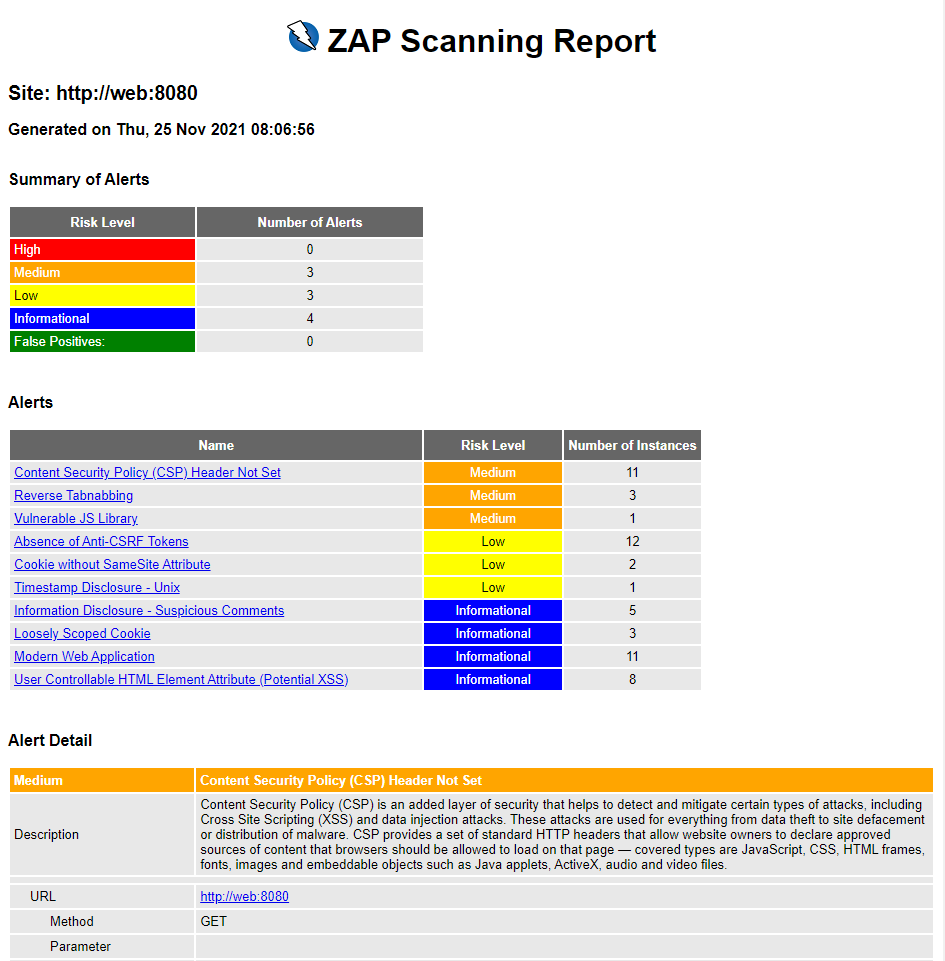
\includegraphics[scale=0.5]{images/zap-report}
    \caption{Bericht nach der Ausführung einer Zap Baseline} \label{fig:baseline}
\end{figure}




Die Sicherheit einer Anwendung zu testen ist eine schwierige Aufgabe,
aber Werkzeuge wie Zap geben vielen Menschen die Möglichkeit, sich in
diesem Bereich leicht einzuarbeiten. Mit Hilfe der Scanner ist es möglich,
Sicherheitslücken zu finden, die den Entwicklern ermöglichen, sie zu
beheben. Dadurch wird eine gute Softwarequalität für die Zukunft gewährleistet.







